\documentclass[11pt]{beamer}
% \usetheme{Boadilla}
  \usetheme{default}


% math mode only
\newcommand {\Lmax} {L_{\mbox{\small max}}}
\newcommand {\Vmax} {V_{\mbox{\small max}}}



\title{interferometric interpolation}
\author{H.~E.~Motteler}
\institute{
  UMBC Atmospheric Spectroscopy Lab \\
  Joint Center for Earth Systems Technology \\
}
\date{\today}
\begin{document}

%----------- slide --------------------------------------------------%
\begin{frame}[plain]
\titlepage
\end{frame}
%----------- slide --------------------------------------------------%
\begin{frame}
\frametitle{basic equations}

The Nyquist equations for Fourier transform interferometry are

\[ \Vmax = n \: dv = 1/ (2\/dx) \]
\[ \Lmax = n \: dx = 1/ (2\/dv) \]

where

\begin{itemize}
  \item $\Lmax$ is maximum OPD
  \item $\Vmax$ is maximum frequency
  \item $dx$ is the distance step
  \item $dv$ is the frequency step
  \item $n$ is the number of steps
% \item the transform size is $2N$
\end{itemize}

\vspace{2mm}
We consider the application to interferometric or ``double Fourier''
interpolation

\end{frame}
%----------- slide --------------------------------------------------%
\begin{frame}
\frametitle{example}

\begin{center}
  \includegraphics[scale=0.4]{figures/cos_tfrm.pdf}
\end{center}

\end{frame}
%----------- slide --------------------------------------------------%
\begin{frame}
\frametitle{discussion}

\begin{itemize}

  \item $\Vmax = n\: dv = 1/(2\/dx)$ and $\Lmax = n\: dx =
    1/(2\/dv)$

  \item $\Lmax$ and $\Vmax$ fall on index $n+1$ when we start
    counting from $1$

  \item index $1$ is optical displacement 0 and index $n+1$ is
    optical displacement $\Lmax$.  We need $n+1$ points to represent
    a full single-sided sweep

  \item starting from spectra we generate the interferogram by
    embedding the spectral interval from $j$ to $k$ in the larger
    zero-filled span from $0$ to $\Vmax$, reflecting this from $n$
    down to $2$ as shown, and doing a $2n$-point inverse FFT

  \item starting from spectra at resolution $dv$, note that choosing
    one of $dx$, $\Vmax$, or $n$ fixes the other values

\end{itemize}

\end{frame}
%----------- slide --------------------------------------------------%
\begin{frame}
\frametitle{discussion}

\begin{itemize}

  \item if our original $n+1$ point spectra is real-valued then the
    interferogram will be as well

  \item the transforms are invertible.  If we start with an $n+1$
    point sweep from $0$ to $\Lmax$, reflect it as shown, and do a
    $2n$ point FFT, we get the spectra and reflection

  \item in practice we might take a $2n$ point sweep from $-\Lmax$
    to $\Lmax$, get an interferogram centered near point $n$, swap
    halves to get something like the interferogram shown, and do a
    $2n$ point FFT to get the spectra and reflection

  \item in that case the resulting spectrum will typically be
    complex, with the imperfect centering appearing as a phase
    shift
    
\end{itemize}

\end{frame}
%----------- slide --------------------------------------------------%
\begin{frame}
\frametitle{interpolation}

\begin{center}
  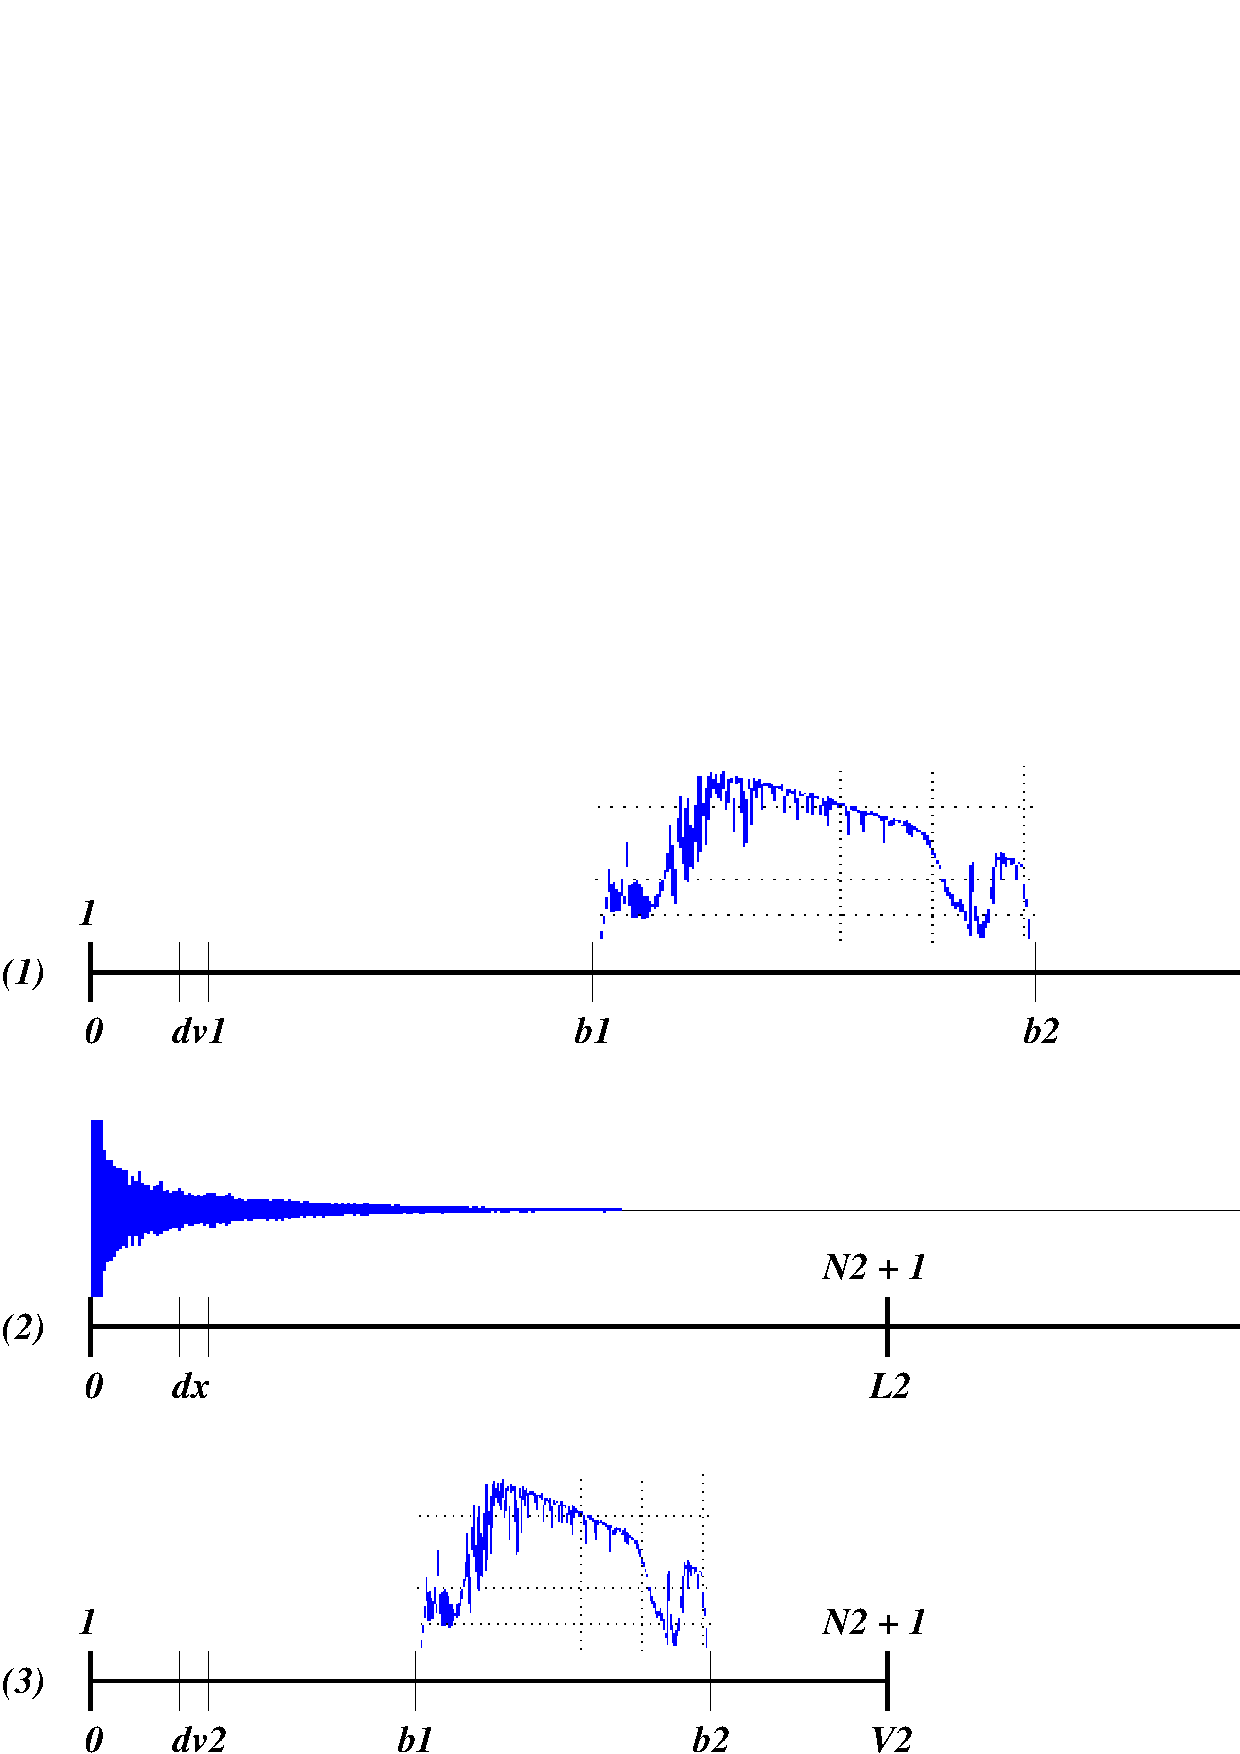
\includegraphics[scale=0.4]{figures/interp_tfrm.pdf}
\end{center}

\end{frame}
%----------- slide --------------------------------------------------%
\begin{frame}
\frametitle{basic equations}

The Nyquist equations for (1) and (2) are

\[ V_1 = N_1 \/dv_1 = 1/(2\/ dx) \]
\[ L_1 = N_1 \/dx   = 1/(2\/ dv_1) \]

and for (2) and (3) are

\[ V_2 = N_2 \/dv_2 = 1/ (2\/ dx) \]
\[ L_2 = N_2 \/dx   = 1/ (2\/ dv_2) \]

If we are given $dv_1$ and $dv_2$ then we need $dx$, $N_1$, or $N_2$
to fill out the values above.  $N_1$ and $N_2$ must be integers.

\end{frame}
%----------- slide --------------------------------------------------%
\begin{frame}
\frametitle{constraints}

Note that $dx$ is the same for both pairs of equations, so $V_1 =
V_2$.  Then $N_1\/dv_1 = N_2\/dv_2$, and we have

\[ N_2 / N_1 = dv_1 / dv_2, \]

a constraint on the transform sizes that can only be satisfied if
$dv_1 / dv_2$ is rational.  In addition, the transforms must include
the band of interest, so we require 

\[ V_1 = N_1\/dv_1 \ge b_2 \]

Suppose $dv_1 / dv_2$ is rational.  Let $m_1$ and $m_2$ be the smallest
integers such that $m_1/m_2 = dv_1 / dv_2$. \\

\end{frame}
%----------- slide --------------------------------------------------%
\begin{frame}
\frametitle{constraints}

Let $k$ be the smallest integer such that $m_2 \cdot 2^k \cdot dv_1
\ge b_2$, and let $N_1 = m_2 \cdot 2^k$ and $N_2 = m_1 \cdot 2^k$. \\
\bigskip
Then the constraints above are satisfied, and in addition if $m_1$
and $m_2$ are not too large then $N_1$ and $N_2$ will have mostly
small prime factors, making the FFT calculation more efficient. \\
\bigskip
If $dv_1 / dv_2$ is not rational or $m_1$ or $m_2$ are very large we
may want to proceed differently, for example by finding a value for
$dv_1$ close to the desired $dv$ but with a more tractible rational
representation.  In that case we might want to do a conventional
interpolation from $dv$ to $dv_1$ as a preliminary step.

\end{frame}
%----------- slide --------------------------------------------------%
\end{document}

